\documentclass[12pt]{article}
\usepackage[utf8]{inputenc}
\usepackage[T2A]{fontenc}
\usepackage[russian]{babel}
\usepackage{amsmath}
\usepackage{amssymb}
\usepackage{dsfont}
\usepackage[dvipsnames]{xcolor}
\usepackage{setspace}
\usepackage{multirow}
\usepackage[a4paper, outer=1.5cm, inner=1.5cm, top=1cm, bottom=1cm]{geometry}
\usepackage{graphicx}
\usepackage{skull}
\usepackage{wasysym}
\usepackage{float}
\graphicspath{{.images/}}
\usepackage{hyperref}
\hypersetup{colorlinks=true, linkcolor=blue, filecolor=magenta, urlcolor=cyan}
\usepackage[firstpage]{draftwatermark}
\SetWatermarkText{
    $\qquad\qquad\qquad\qquad\qquad$\parbox{7cm}{\begin{center}
    
\includegraphics[width = 0.08\textwidth]{lion-logo.png}\bigskip\\~\bigskip\\~\vspace{-24mm}\\~\end{center}}
}
\SetWatermarkAngle{0}
\SetWatermarkScale{1.5}
\usepackage{etoolbox}

\newtoggle{ifsolved}
\newtoggle{needhelp}
\newcounter{num}
\setcounter{num}{1}

\newcommand{\newnum}{\par\textbf{\textnumero\arabic{num}}\stepcounter{num}}
\newcommand{\sol}{\vspace{3mm}\par\textbf{Решение: }}
\newcommand{\ans}{\vspace{3mm}\par\textbf{Ответ: }}
\newcommand{\hint}{\vspace{3mm}\par\textbf{Подсказка: }}
\newcommand{\mode}[1]{
\ifstrequal{#1}{0}{\togglefalse{ifsolved}\togglefalse{needhelp}}{\ifstrequal{#1}{1}{\togglefalse{ifsolved}\toggletrue{needhelp}}{\ifstrequal{#1}{2}{\toggletrue{ifsolved}\togglefalse{needhelp}}{\toggletrue{ifsolved}\toggletrue{needhelp}}}}} %if 0 - if 1 - if 2 - else
%\newenvironment{problem}[8]{%#1, #2, #3
%\parbox{\linewidth}{\vspace{4mm}\ifstrequal{#4}{(лёгкая)}{\newnum\textbf{.}}{\newnum\textbf{*.} } \\ #5}
%\iftoggle{ifsolved}{\sol #6}{}
%\iftoggle{ifsolved}{\ans #7}{}
%\iftoggle{needhelp}{\hint #8}{}}

\newenvironment{problem}[8]{%#1, #2, #3
\parbox{\linewidth}{\vspace{5mm}\ifstrequal{#4}{(лёгкая)}{\newnum\textbf{.}}{\newnum\textbf{*.} } \\ #5}
\iftoggle{ifsolved}{\sol #6}{}

\iftoggle{ifsolved}{\parbox{\linewidth}{\ans #7}}{}
\iftoggle{needhelp}{\parbox{\linewidth}{\hint #8}}{}}

\newenvironment{mylist} %custom list
{ \begin{itemize}
    \setlength{\itemsep}{0pt}
    \setlength{\parskip}{0pt}
    \setlength{\parsep}{0pt}     }
{ \end{itemize}                  }

\newenvironment{homeass}[1]{\vspace*{-1.5cm}
\iftoggle{ifsolved}{
    \section*{\center{Решение домашнего задания к #1.}}
}{
    \section*{\center{\textcolor{Sepia}{Домашнее задание к #1}}}
} \vspace{7mm}\large}

\parindent=0pt
\pagestyle{empty}
%$\!$[\arabic{class}.\arabic{num}]
%\ifnumcomp{\value{counter}}{>}{1}{true}{false}
%\definecolor{Gray}{gray}{0.9}
%\definecolor{mypink}{RGB}{219, 48, 122}
%\newcolumntype{g}{>{\columncolor{Gray}}p{2.8cm}}

\begin{document}
\large
\mode{7}
%0 for problems without hints
%1 for problems + hints
%2 for problems + solutions + answers
%else: show all

{\centering\section*{СПИСОК ЗАДАЧ}}

{\centering\subsection*{\smallskip\\\textcolor{green}{\textbf{Полезные вещи, которые можно и нужно копипастить:}}}}

\subsection*{\textcolor{Emerald}{\textbf{Полезные шпаргалки по LaTeXу:}}}

\textbf{Пример вставки рисунка:}

\begin{minipage}{\linewidth}
    \begin{minipage}{0.54\linewidth}
    см. рисунок справа\\
    Текст к собственно пикче, примерно всегда это либо развёрнутое описание, либо большая часть решения задачи --- стремимся экономить пространство, если это можно сделать.
    \end{minipage}
    \hspace{0.05\linewidth}
    \begin{minipage}{0.4\linewidth}
    \begin{figure}[H] 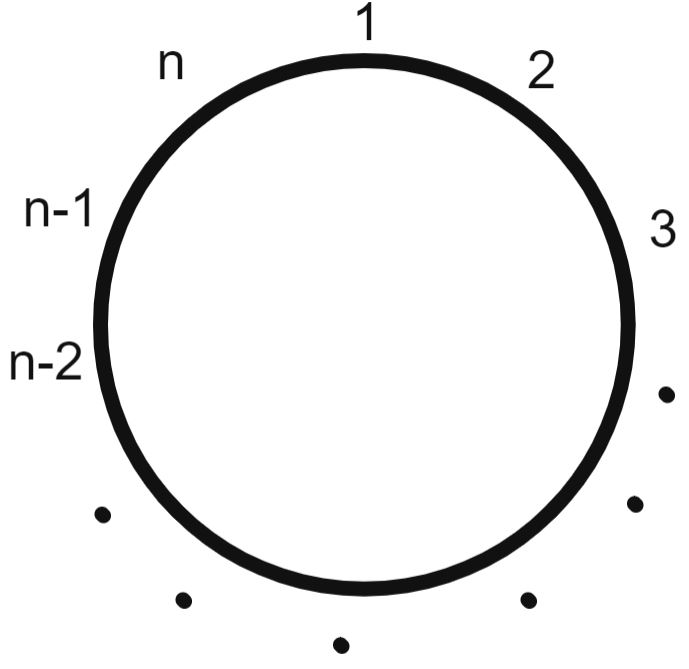
\includegraphics[width=\linewidth]{sol3} %тут поменять имя пикчи
    \end{figure}
    \end{minipage}
\end{minipage}

\textbf{Дефолтные математические знаки и символы:}\\
$\geqslant$,
$\leqslant$,
$a^{b}$,
$x_{i}$,
$\sqrt{a}$,
$\frac{a}{b}$,
$\displaystyle \frac{a}{b}$,
$\cdot$
$\;\Rightarrow\;$,
$\;\Leftrightarrow\;$,
$1{,}2$.
О промежутках:
$a\!b$,
$a\,b$,
$a\:b$,
$a\;b$,
$a\quad b$.

\textbf{Стандартные система и совокупность уравнений / неравенств:}\\
$\left\{
\begin{aligned}
f(x) &= 0 \\
g(x) &= 1
\end{aligned}\right.$

$\left[\begin{aligned}
&\left\{\begin{aligned}
f(x) &\geqslant a \\
g(x) &= b
\end{aligned}\right.\\
&\left\{\begin{aligned}
f(x) &< a \\
g(x) &= -b
\end{aligned}\right.
\end{aligned}\right.$

\subsection*{\textcolor{Emerald}{\textbf{Не математическое, но полезное:}}}
% комментарий в любом месте документа, который нигде не будет видно. Можно использовать для написания заметок-вопросов по задачам
\textbf{Пример таблицы:}

\begin{tabular}{|c|c|c|}
\hline
    $a$ & $b$ & текст
\\\hline
    $c$ & $d$ & мораль
\\\hline
\end{tabular}\\

\textbf{Отступы:} между\smallskip\\ строками\medskip\\ \textbf{Тире} --- это три дефиса.\\
\textbf{Списки:}
\begin{mylist}
\item [$\bullet$] это был пункт а
\item [2)] а это уже пункт номер 2 с изменённым заголовком
\end{mylist}

\subsection*{\textcolor{Emerald}{\textbf{Всё, неупомянутое выше (или если просто что-то не так):}}}
\begin{mylist}
\item [$\bullet$] Решение отдельных вопросов касательно ТеХа нужно искать в \href{https://www.mccme.ru/free-books/llang/newllang.pdf}{Львовском}.

\item [$\bullet$] Найти произвольный символ, который нужен, можно в \href{http://detexify.kirelabs.org/classify.html}{Detexify}.

\item [$\bullet$] Если возникли сомнения при решении, ответ практически ко всем задачам можно проверить с помощью \href{https://www.wolframalpha.com/}{WolframAlpha}.

\item [$\bullet$] Если в задаче нужно создать картинку, то лучше пока отложить эту задачу. Все графики планируется централизованно нарисовать (или перерисовать) в геогебре.

\item [\textcolor{brown}{\textbf{!!}}] Важно ставить \textcolor{red}{\textbf{$\spadesuit$}}
(или просто red) в тело задачи в случае серьёзных вопросов к решению и какой-то вопиющей лажи.

\item [\textcolor{brown}{\textbf{!!}}] Важно ставить \textcolor{olive}{\textbf{$\spadesuit$}}
(или просто olive) в тело задачи в случае не самого удачного текста и кривых отступов.
\end{mylist}

\subsection*{\textcolor{Violet}{\textbf{Комментарии:}}}% а также невидимые комментарии - так можно оставлять заметки-вопросы прямо в задаче, чтобы потом было понятно, в чём вопрос.
\begin{mylist}
\item [$\skull$] Переставлять задачи местами --- очень плохая идея.

\item [$\smiley$] При двойном клике по тексту pdf справа происходит автоматический переход к этому месту в латех-коде, а для обратного перехода можно нажать стрелку вправо (висит сверху между pdf и латех-кодом).

\item [$\smiley$] Если есть размышления, дописывать red/olive к задаче или не дописывать, то лучше всё-таки дописать.

\item [$\skull$] Самое плохое, что можно сделать --- написать в любое поле из трёх (НаписанноеРешение/ВерныйОтвет/Подсказка) только половину того, что надо, никак это не отметить, и потом пойти дальше.\\ Нужно в этот момент писать red/olive в случайном месте задачи, чтобы потом вычислить это с помощью Ctrl+F по всему документу (и это то, что потом будет делаться долго и тщательно)
\end{mylist}

\newpage
\setcounter{num}{801}

\hypertarget{8.1}{{\centering\section*{\bigskip\\\textcolor{Blue}{\hyperlink{start2}{\textcolor{Blue}{8.1}} График линейной функции.}\vspace{-5mm}}}}

\begin{problem}{Декартова система координат и линии на ней.}{8.1.2}{6K}{(лёгкая)}
{Придумать несколько решений уравнения $x + 2y = 3$ (не обязательно целых). Нарисовать точки с такими координатами $(x; y)$ на координатной плоскости (например, $(7; -2))$. Что получилось? Почему?}
{НаписанноеРешение}
{ВерныйОтвет}{Подсказка}
\end{problem}

\begin{problem}{Линейное уравнение с двумя неизвестными, график прямой.}{8.1.3}{6K}{*}
{a) Придумать любые две пары целых чисел, меньших 10 (например: 1, 4 и 6, $-6$);
\\b) Нарисовать две точки с этими координатами (в моём случае это $(1; 4)$ и $(6; -6)$);
\\c) Провести через них прямую и найти уравнение, соответствующее этой прямой (для указанных в примере точек это будет уравнение $y = -2x + 6$)}
{Приведу решение для любых задуманных чисел: допустим, были задуманы какие-то четыре числа $a$, $b$, $c$, $d$. Мы знаем, что получившиеся две точки $(a; b)$ и $(c; d)$ лежат на какой-то пока неизвестной нам прямой $y = kx + p$.\\ Наша задача~--- найти числа $k$ и $p$ (тогда и уравнение прямой будет найдено, и нарисовать прямую мы сможем). Но раз мы знаем, что точка $(a; b)$ находится на этой прямой, то из $y = kx + p$ получается уравнение $b = ka + p$. Аналогичным образом получается $d = kc + p$. Вычтем из первого уравнения второе: $b - d = (ka + p) - (kc + p) \;\Rightarrow\; b - d = ka - kc \;\Rightarrow\; b - d = (a - c)k \;\Rightarrow\; k = \frac{b - d}{a - c}$.\\
Мы нашли $k$ (ведь теперь значение дроби можно вычислить: $a$, $b$, $c$, $d$ известны).\\
Теперь можно и $p$ найти: $b = ka + p \;\Rightarrow\; p = b - ka = b - \frac{b - d}{a - c} \cdot a$. Готово.\\ Можно и немного упростить: $p = b - \frac{b - d}{a - c} \cdot a = b\cdot \frac{a - c}{a - c} - a \cdot \frac{b - d}{a - c} = \frac{ba - bc - (ab - ad)}{a - c} = \frac{ad - bc}{a - c}$.\\
Итого, какие бы четыре числа $a$, $b$, $c$, $d$ не были загаданы, $k = \frac{b - d}{a - c}$, $\,p = \frac{ad - bc}{a - c}$.\\ Вот несколько примеров (разных ($a$, $b$, $c$, $d$)) и график всех этих прямых:\\
\begin{tabular}{|c|c|c|c|c|c|c|c|}
\hline
    $a$ & $b$ & $c$ & $d$ & $\!(a; b)$ и $(c; d)\!$ & $\vphantom{\Bigr(} k = \frac{b - d}{a - c}$ & $p = \frac{ad - bc}{a - c}$ & $y = kx + p$\\\hline
    $5$ & $7$ & $\!-3\!$ & $\!-1\!$ & \textcolor{Blue}{$(5; 7)$} и \textcolor{Blue}{$(-3; -1)$} & $\vphantom{\Bigr(} \frac{7-(-1)}{5-(-3)} = 1$ & $\frac{5(-1) - 7(-3)}{5-(-3)} = 2$ & \textcolor{Blue}{$y = x + 2$} \\\hline
    $4$ & $2$ & $0$ & $\!-2\!$ & \textcolor{BrickRed}{$(4; 2)$} и \textcolor{BrickRed}{$(0; -2)$} & $\vphantom{\Bigr(} \frac{2-(-2)}{4-0} = 1$ & $\frac{4(-2) - 2\cdot0}{4-0} = -2$ & \textcolor{BrickRed}{$y = x - 2$} \\\hline
    $\!-4\!$ & $6$ & $1$ & $\!-9\!$ & \textcolor{Orange}{$(-4; 6)$} и \textcolor{Orange}{$(1; -9)$} & $\vphantom{\Bigr(} \frac{6-(-9)}{-4-1} = -3$ & $\frac{(-4)(-9) - 6\cdot1}{-4-1} = -6$ & \textcolor{Orange}{$y = -3x - 6$} \\\hline
    $1$ & $\!-1\!$ & $5$ & $\!-1\!$ & \textcolor{CadetBlue}{$(1; -1)$} и \textcolor{CadetBlue}{$(5; -1)$} & $\vphantom{\Bigr(} \frac{-1-(-1)}{1-5} = 0$ & $\frac{1\cdot(-1) - (-1)\cdot5}{1-5} = -1$ & \textcolor{CadetBlue}{$y = -1$} \\\hline
    $\!-3\!$ & $3$ & $\!-6\!$ & $4$ & \textcolor{OliveGreen}{$(-3; 3)$} и \textcolor{OliveGreen}{$(-6; 4)$} & $\!\vphantom{\Bigr(} \frac{3-4}{(-3)-(-6)} = -\frac13\!$ & $\frac{(-3)\cdot 4 - 3(-6)}{(-3)-(-6)} = 2$ & \textcolor{OliveGreen}{$y = -\frac13 x + 2$} \\\hline
    $6$ & $0$ & $\!-9\!$ & $5$ & \textcolor{LimeGreen}{$(6; 0)$} и \textcolor{LimeGreen}{$(-9; 5)$} & $\vphantom{\Bigr(} \frac{0-5}{6-(-9)} = -\frac13$ & $\frac{6\cdot 5 - 0\cdot(-9)}{6-(-9)} = 2$ & \textcolor{OliveGreen}{$y = -\frac13 x + 2$} \\\hline
    $\!-5\!$ & $\!-7\!$ & $7$ & $2$ & \textcolor{Orchid}{$(-5; -7)$} и \textcolor{Orchid}{$(7; 2)$} & $\vphantom{\Bigr(} \frac{(-7)-2}{(-5)-7} = \frac34$ & $\!\frac{(-5)\cdot 2 - (-7)\cdot7}{(-5)-7} = -\frac{13}{4}\!$ & \textcolor{Orchid}{$y = \frac34 x - \frac{13}{4}$} \\\hline
\end{tabular}\vspace{-3mm}\\
\begin{center}
\begin{minipage}{0.75\linewidth}
    \begin{figure}[H]
    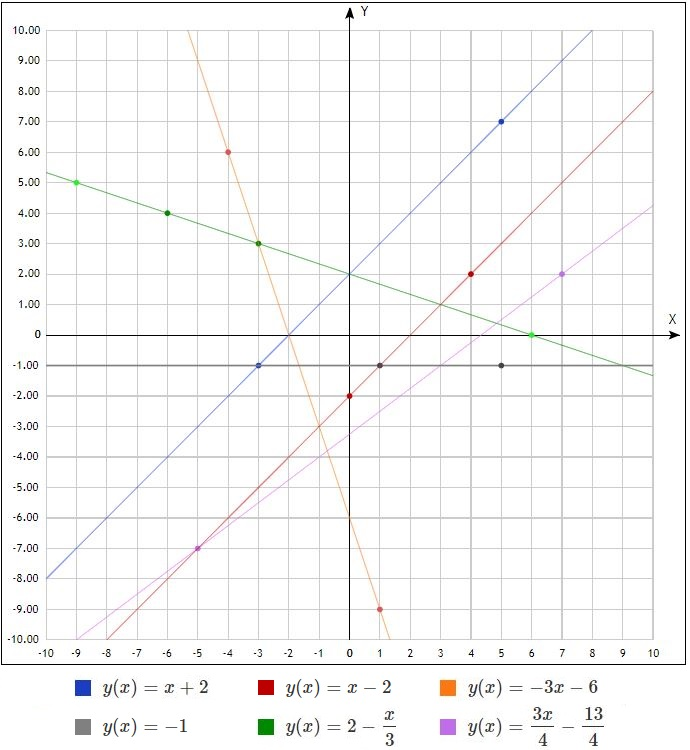
\includegraphics[width=\linewidth]{sol32}
    \end{figure}
\end{minipage}
\end{center}
}
{Смотри рисунок выше. Уравнение прямой имеет вид $y = \frac{b - d}{a - c}\cdot x + \frac{ad - bc}{a - c}$.}{Пусть уравнение искомой прямой имеет вид $y = kx + b$. Какое уравнение можно получить, если известно, что точка $(x_0; y_0)$ лежит на этой прямой?}
\end{problem}

\begin{problem}{Линейное уравнение с двумя неизвестными, график прямой.}{8.1.3}{7A}{(лёгкая)}
{Найти уравнение прямой, проходящей через точки $(-1; 2)$ и $(2; 1)$.}
{НаписанноеРешение}
{ВерныйОтвет}{Подсказка}
\end{problem}

\begin{problem}{Линейное уравнение с двумя неизвестными, график прямой.}{8.1.3}{7A}{(лёгкая)}
{При каком значении $a$ точка $B (a + 1; a - 2)$ принадлежит прямой $y + a + 7 - x = 0$?

}
{НаписанноеРешение}
{ВерныйОтвет}{Подсказка}
\end{problem}

\begin{problem}{Линейное уравнение с двумя неизвестными, график прямой.}{8.1.3}{7A}{(лёгкая)}
{Найти расстояние до оси $y$ от точки пересечения прямых $2x + y = 1$ и $x + 2y = 1$.

}
{\vspace{-6mm}\\\begin{minipage}{\linewidth}
    \begin{minipage}{0.47\linewidth}
    ~\vspace{1mm}\\
    Первая прямая~--- то же самое, что и прямая $y = 1 - 2x$, уравнение же для второй прямой можно переписать как $2y = 1 - x$, откуда $y = \frac{1 - x}{2}$.\\
    Первую прямую можно построить по паре точек $(0; 1)$ и $(\frac12; 0)$, а вторую~--- по паре точек $(0; \frac12)$ и $(1; 0)$.\smallskip\\
    Полученные прямые изображены на графике справа.\medskip\\
    Точка пересечения не находится на координатной сетке, поэтому нужно задействовать алгебраический способ, чтобы найти её координаты:
    
    \end{minipage}
    \hspace{0.05\linewidth}
    \begin{minipage}{0.48\linewidth}
        \begin{figure}[H]
        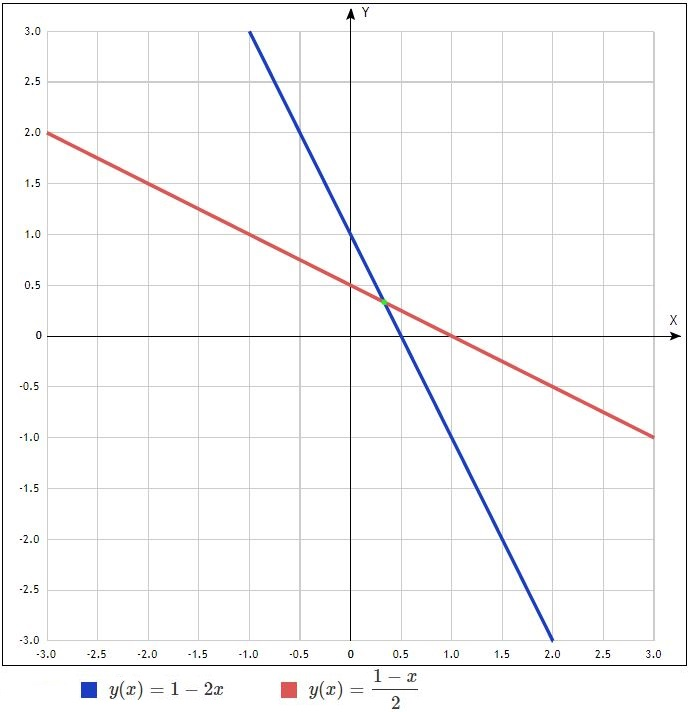
\includegraphics[width=\linewidth]{sol30}
        \end{figure}
    \end{minipage}
\end{minipage}
$1 - 2x = y = \frac{1 - x}{2} \;\Rightarrow\; 1 - 2x = \frac{1 - x}{2} \;\Rightarrow\; 2 - 4x = 1 - x \;\Rightarrow\; 1 = 3x \;\Rightarrow\; x = \frac13$.\\
Значит, у точки пересечения $x$-координата равна $\frac13$.\\ Следовательно, её $y$-координата равна $y = 1 - 2x = 1 - 2\cdot\frac13 = \frac13$. Точка $(\frac13; \frac13)$ находится на расстоянии $\frac13$ и от оси $y$, и от оси $x$. Таким образом, ответ~--- $\frac13$.}
{Расстояние от точки пересечения этих прямых до оси $y$ равно $\frac13$.}{В точке пересечения у обоих прямых одно и то же значение $y$.}
\end{problem}

\begin{problem}{Линейное уравнение с двумя неизвестными, график прямой.}{8.1.3}{7A}{(лёгкая)}
{При каких значениях $p$ расстояние от точки пересечения прямых $y - px = 0$ и $x + 2y = 1$ до оси $x$ будет равно 1?}
{НаписанноеРешение}
{ВерныйОтвет}{Подсказка}
\end{problem}

\begin{problem}{Линейная функция на множестве.}{8.1.4}{6K}{*}
{Мама послала семилетнего Васю в магазин купить хлеб.\\ Вася настроился очень серьезно, не забыл взять с собой все свои деньги~--- много двух- и пяти- рублёвых монет, но перенервничал и забыл, что ему могут дать сдачу. Сколько монет ему пришлось отдать, если хлеб стоил 31 рубль, а он заплатил за него без сдачи?}
{НаписанноеРешение}
{ВерныйОтвет}{Подсказка}
\end{problem}

\begin{problem}{Прямая пропорциональность и её график.}{8.1.5}{6S}{(лёгкая)}
{Пассажирский поезд проходит расстояние между двумя городами за 10 ч, а товарный поезд это же расстояние проходит за 15 ч.\\ Оба поезда одновременно вышли из городов навстречу друг другу.\\ Через сколько часов они встретятся? Решить задачу графически.}
{\vspace{-9mm}\\\begin{minipage}{\linewidth}
    \begin{minipage}{0.39\linewidth}
    \vspace{11mm}
    Изобразим график движения поездов: по одной оси отложим время, а по другой~--- расстояние от города, откуда вышел пассажирский поезд (в частях от общего расстояния $s$).
    \end{minipage}
    \hspace{0.02\linewidth}
    \begin{minipage}{0.58\linewidth}\begin{figure}[H] 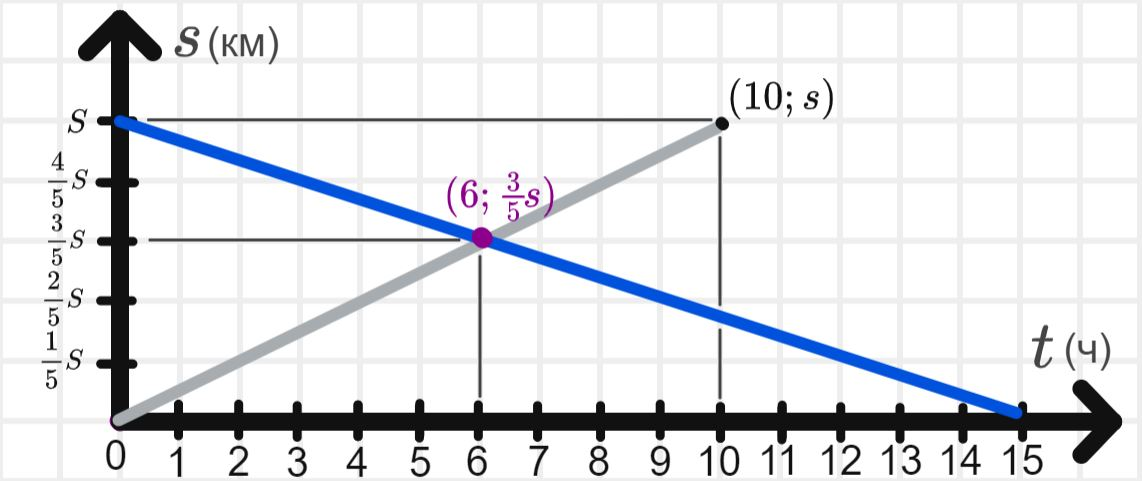
\includegraphics[width=\linewidth]{sol10}\end{figure}\end{minipage}
\end{minipage}
\vspace{-1mm}\\Как видно из рисунка, пересечение происходит спустя 6 часов после начала движения. Поскольку в этот момент расстояние от каждого поезда до первого города одно и то же, это момент встречи. То же самое без помощи графиков:\\ скорость сближения равна $\frac{1}{10} + \frac{1}{15} = \frac{3 + 2}{30} = \frac16 \;\Rightarrow$ они встретятся через 6 часов.}
{Поезда встретятся через 6 часов.}{Общее расстояние по вертикальной оси измеряется в частях $s$.}
\end{problem}

\begin{problem}{Различные коэффициенты линейных функций, расположение прямых на графике.}{8.1.6}{6K}{(лёгкая)}
{(Крутимся-вертимся) Нарисовать на одной и той же плоскости те точки $(x; y)$, для которых верно:
\\a) $y = 3x$ (то есть, например $(1; 3)$, $(2; 6)$, $(-\frac{1}{3}; -1)$; \hfill b) $y = x$;
\\c) $y = x/2$; \hfill d) $y = x/5$.
\\На другой плоскости рядом с предыдущей нарисовать точки $(x; y)$, для которых верно:
\\e) $y = 3x + 2$; \hfill f) $y = x + 2$;
\\g) $y = x/2 + 2$; \hfill h) $y = x/5 + 2$.\\
Какие выводы можно сделать для прямой $y = ax + b$?\hfill ($a$ и $b$~--- какие-то числа)}
{Нарисуем все прямые по точкам и сравним результаты: \vspace{-5mm}\\\begin{minipage}{\linewidth}
    \begin{minipage}{\linewidth}\begin{figure}[H] 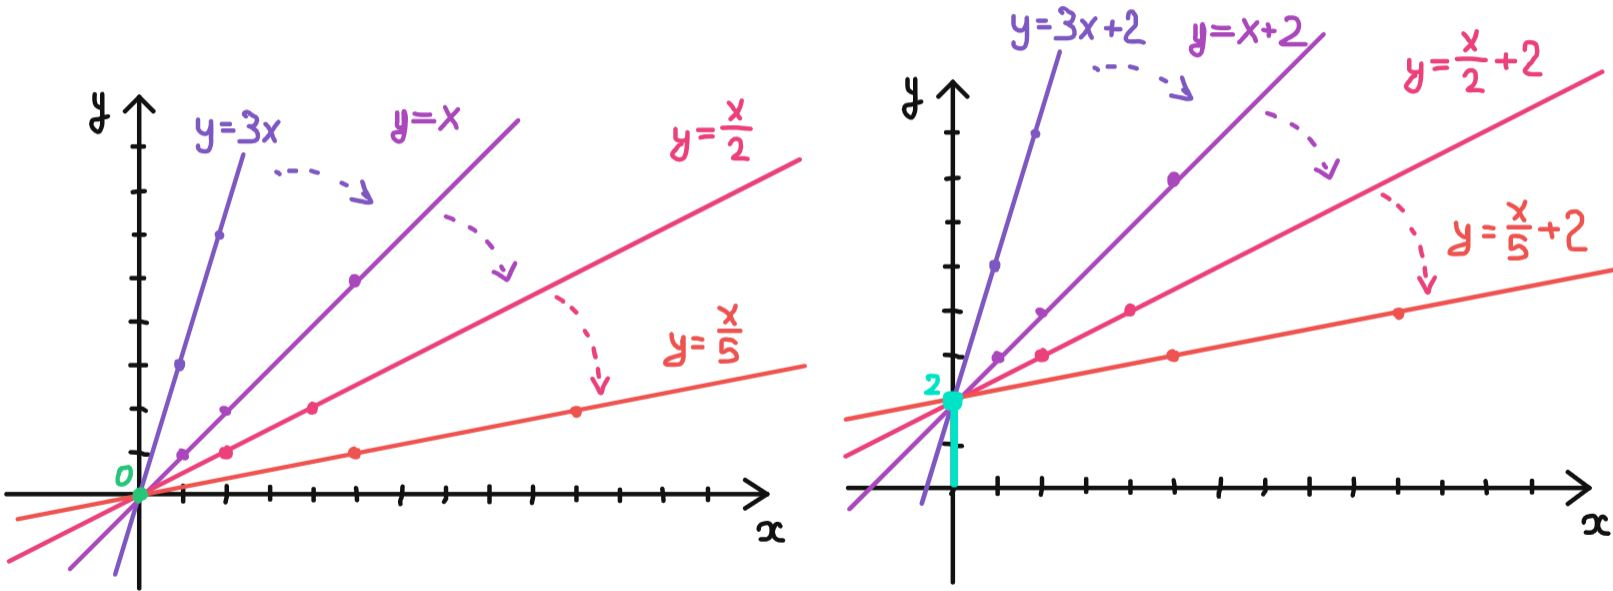
\includegraphics[width=\linewidth]{sol12}\end{figure}\end{minipage}
\end{minipage}
Первые 4 прямых все проходят через точку $(0; 0)$, и каждая следующая прямая положе предыдущей (это так, потому что $3 < 1 < \frac12 < \frac15$).
Вторая же четвёрка прямых~--- это те же самые прямые, но к которым прибавили 2. Поэтому вся картинка просто находится на 2 выше~--- больше ничего не меняется.\\
Таким образом, можно сделать следующий вывод: у прямой $y = ax + b$ число $b$ отвечает за то, насколько нужно сдвинуть график вверх-вниз (если $b$ отрицательно, то вниз). А коэффициент при $x$, число $a$ отвечает за пологость~--- чем меньше $a$, тем более пологой будет прямая (отмечу, что это мы утверждаем только для положительных $a$).}
{У прямой $y = ax + b$ число $a$ показывает крутизну прямой, а $b$~--- сдвиг.

}{Нужно сделать выводы про наклон и сдвиги.}
\end{problem}

\begin{problem}{Различные коэффициенты линейных функций, расположение прямых на графике.}{8.1.6}{6K}{(лёгкая)}
{Нарисовать на одной плоскости графики прямых $y = x + 2$, $\,y = 5 - 2x$, $\,y = \frac{1 - x}{2}$.\\
Найти координаты всех точек пересечения.}
{Построим графики всех прямых по парам точек:\\ Для первой прямой это пара точек $(0; 2)$ и $(1; 3)$.\\
Для второй прямой~--- точки $(1; 3)$ и $(2; 1)$.\\
Для третьей прямой~--- точки $(1; 0)$ и $(3; -1)$.\vspace{-3mm}\\\begin{minipage}{\linewidth}
    \begin{minipage}{0.47\linewidth}
    Полученные прямые изображены на графике справа.\bigskip\\
    Точки пересечения при хорошем чертеже должны быть видны невооружённым глазом: это точки $(-1; 1)$, $(1; 3)$, $(3; -1)$.\smallskip\\
    Однако есть способ, как найти точки пересечения алгебраически (полезен, если точки пересечения находятся не на координатной сетке).\bigskip\\
    Приведу и алгебраическое решение:
    
    \end{minipage}
    \hspace{0.05\linewidth}
    \begin{minipage}{0.48\linewidth}
        \begin{figure}[H]
        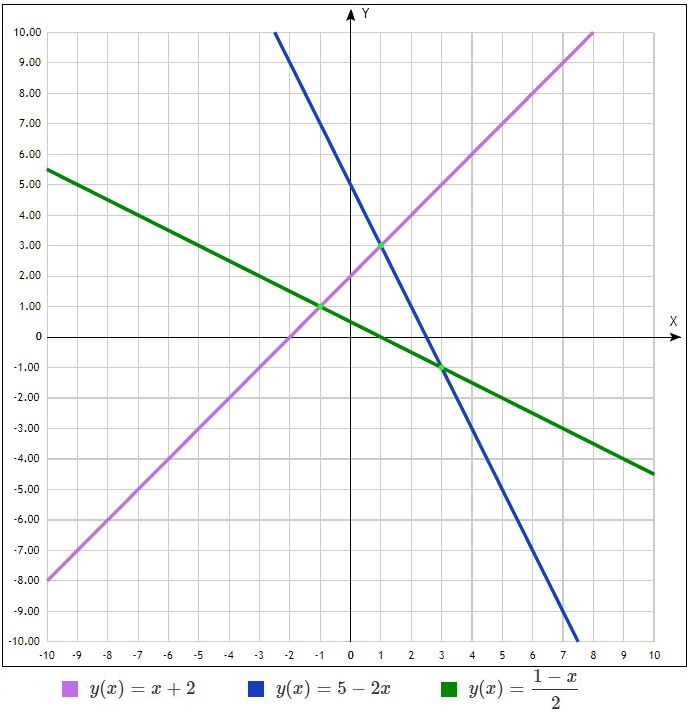
\includegraphics[width=\linewidth]{sol29}
        \end{figure}
    \end{minipage}
\end{minipage}
Найдём точку пересечения первой и второй прямой: $x + 2 = y$; $\,y = 5 - 2x \;\Rightarrow\;$\\
$x + 2 = 5 - 2x \;\Rightarrow\; 3x = 3 \;\Rightarrow\; x = 1 \;\Rightarrow\; y = 1 + 2 = 3$.\\ Таким образом, $(1;\, 3)$~--- точка пересечения первой и второй прямой.\\
Первая и третья прямая: $x + 2 = y = \frac{1 - x}{2} \;\Rightarrow\; 2x + 4 = 1 - x \;\Rightarrow\; 3x = -3 \;\Rightarrow\; x = -1 \;\Rightarrow\; y = -1 \!+\! 2 = 1 \;\Rightarrow\; (-1; 1)$~--- точка пересечения первой и третьей прямой.\\
Вторая и третья: $5 - 2x = y = \frac{1 - x}{2} \;\Rightarrow\; 10 - 4x = 1 - x \;\Rightarrow\; 9 = 3x \;\Rightarrow\; x = 3 \;\Rightarrow\; y = \frac{1 - 3}{2} = -1 \;\Rightarrow\;$ точка $(3; -1)$~--- точка пересечения второй и третьей прямой.}
{Графики прямых изображены на рисунке выше. \\
Координаты точек пересечения~--- $(1;\, 3)$, $(-1;\, 1)$, $(3; -1)$.}{Достаточно аккуратно нарисовать все прямые по точкам.}
\end{problem}

\begin{problem}{Различные коэффициенты линейных функций, расположение прямых на графике.}{8.1.6}{6K}{(лёгкая)}
{Нарисовать на одной плоскости графики прямых $4y = 3x + 4$, $4y = 3x + 9$, $4y = 3x + 14$, $4y = 3x + 19$, $4y = 3x + 24$. Нарисовать на том же графике\\ прямые $3y + 4x = 3$, $3y + 4x = 8$, $3y + 4x = 13$, $3y + 4x = 18$, $3y + 4x = 23$.}
{НаписанноеРешение}
{ВерныйОтвет}{Подсказка}
\end{problem}

\begin{problem}{Различные коэффициенты линейных функций, расположение прямых на графике.}{8.1.6}{6K}{(лёгкая)}
{Нарисовать на клетчатой бумаге четыре прямых: $3y = 4x;\;$ $4y = -3x;$\\ $3y = 4x - 25;\;$ $4y = -3x + 25,\;$ найти точки их пересечения (4 штуки).\\ Найти площадь фигуры, которую образуют эти прямые.\\
Выяснить, чему равны её стороны (потом проверить себя с помощью линейки).

}
{\vspace{-5mm}\\\begin{minipage}{\linewidth}
    \begin{minipage}{0.51\linewidth}
    \vspace{7mm}
    Смотри рисунок справа: данные прямые, построенные по точкам, образуют квадрат с вершинами в точках пересечения~--- $(0; 0)$, $(3; 4)$, $(7; 1)$, $(4; -3)$.\smallskip\\
    (отмечу, что строгого доказательства \\ того что это квадрат, у нас всё ещё нет.)\smallskip\\
    Если посчитать площадь всех клеточек внутри этой фигуры, то мы получим 25, то есть площадь квадрата равна 25 квадратным клеткам, а значит, его сторона должна быть равна 5 клеткам.\\ Можно проверить с помощью линейки.
    \end{minipage}
    \hspace{0.05\linewidth}
    \begin{minipage}{0.43\linewidth}\begin{figure}[H] 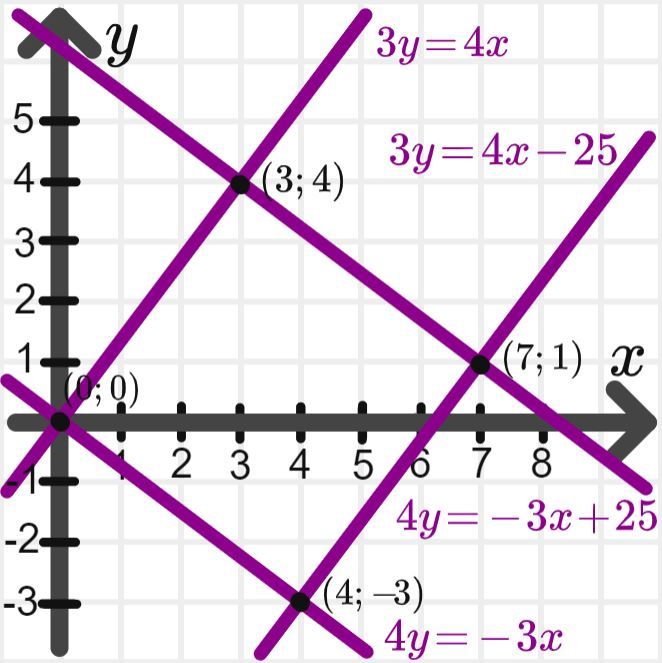
\includegraphics[width=\linewidth]{sol11}\end{figure}\end{minipage}
\end{minipage}}
{Получается квадрат со стороной 5; точки пересечения прямых~--- точки $(0; 0)$, $(3; 4)$, $(7; 1)$, $(4; -3)$.}{Получится квадрат, а чтобы посчитать его площадь, можно посчитать число клеточек внутри.}
\end{problem}

\begin{problem}{Решение системы линейных уравнений графическим методом.}{8.1.7}{7A red параметр}{(лёгкая)}
{При каком значении параметра $c$ прямые $3x + 2y = 1$, $3x + 4y = 5$, $6x + cy = c$ пересекаются ровно дважды?}
{НаписанноеРешение}
{ВерныйОтвет}{Подсказка}
\end{problem}

\begin{problem}{Решение системы линейных уравнений графическим методом.}{8.1.7}{7A red параметр}{(лёгкая)}
{При каком значении параметра $a$ прямые $4x - 2y = 7$ и $ax = a - 4y$ не пересекаются?}
{НаписанноеРешение}
{ВерныйОтвет}{Подсказка}
\end{problem}

\begin{problem}{Решение системы линейных уравнений графическим методом.}{8.1.7}{7A red параметр}{(лёгкая)}
{При каком значении параметра $b$ прямые $3x + 2y = 5$ и $bx = b - 4y$ не пересекаются?

}
{НаписанноеРешение}
{ВерныйОтвет}{Подсказка}
\end{problem}

\begin{problem}{Решение системы линейных уравнений графическим методом.}{8.1.7}{7A}{(лёгкая)}
{Первая прямая проходит через точки $(0; 4{,}5)$ и $(3; 6)$. Вторая прямая проходит через точки $(1; 2)$ и $(-4; 7)$. Найти координаты общей точки этих двух прямых.}
{НаписанноеРешение}
{ВерныйОтвет}{Подсказка}
\end{problem}

\begin{problem}{Решение системы линейных уравнений графическим методом.}{8.1.7}{7A}{*}
{Нарисовать на графике прямые $y = \frac{x}{3} + 1$ и $y = 11 - 3x$, найти точку пересечения этих прямых. Найти угол между этими двумя прямыми.}
{\vspace{-5mm}\\\begin{minipage}{\linewidth}
    \begin{minipage}{0.51\linewidth}
    \vspace{8mm}
    Прямые изображены на рисунке справа.\smallskip\\
    Отмечу, что для построения первой прямой удобно взять $x = 0$ и $x = 3$, а для второй прямой~--- $x = 1$ и $x = 2$ (и вообще для прямых можно выбирать точки так, чтобы вычисления были проще).\smallskip\\
    Точку пересечения $(3; 2)$ можно получить и с помощью методов алгебры: действительно, если точка пересечения имеет координаты $(x_0; y_0)$, то $\frac{x_0}{3} + 1 = y_0 = 11 - 3x_0$.\\
    Тогда $\frac{x_0}{3} + 1 = 11 - 3x_0 \;\Rightarrow\; \frac{10x_0}{3} = 10 \;\Rightarrow$ \\ $\Rightarrow x_0 = 3 \;\Rightarrow\; y_0 = 11 - 3\cdot3 = 2$.
    \end{minipage}
    \hspace{0.05\linewidth}
    \begin{minipage}{0.43\linewidth}\begin{figure}[H] 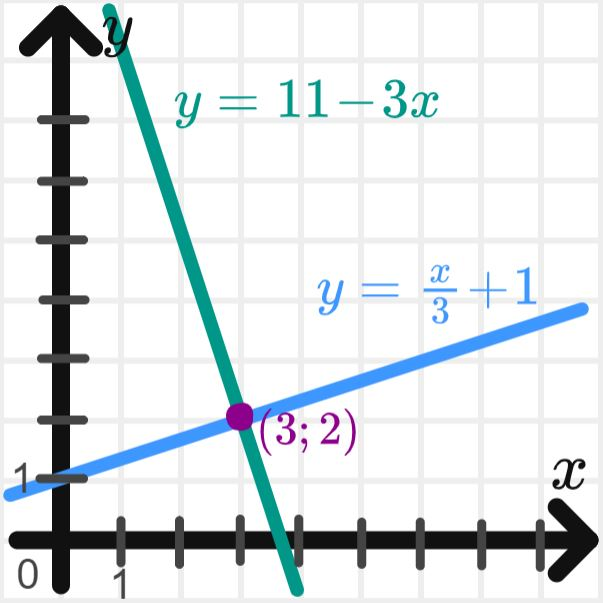
\includegraphics[width=\linewidth]{sol13}\end{figure}\end{minipage}
\end{minipage}
\vspace{-5mm}\\\begin{minipage}{\linewidth}
    \begin{minipage}{0.51\linewidth}
    \vspace{7mm}
    Из рисунка видно, что прямые перпендикулярны, однако докажем это строго.\smallskip\\
    Обозначим точки $O$, $A_1$, $A_2$, $B_1$, $B_2$ как показано на рисунке справа, и нарисуем треугольники $OA_1B_1$ и $OA_2B_2$.\\ В результате стороны треугольников $OB_1 = OB_2 = 3$, $A_1B_1 = A_2B_2 = 1$, и полученные треугольники будут абсолютно одинаковыми (это связано с тем, что у одной прямой коэффициент при $x$ равен $\frac13$, а у другой $-3$).
    \end{minipage}
    \hspace{0.05\linewidth}
    \begin{minipage}{0.43\linewidth}\begin{figure}[H] 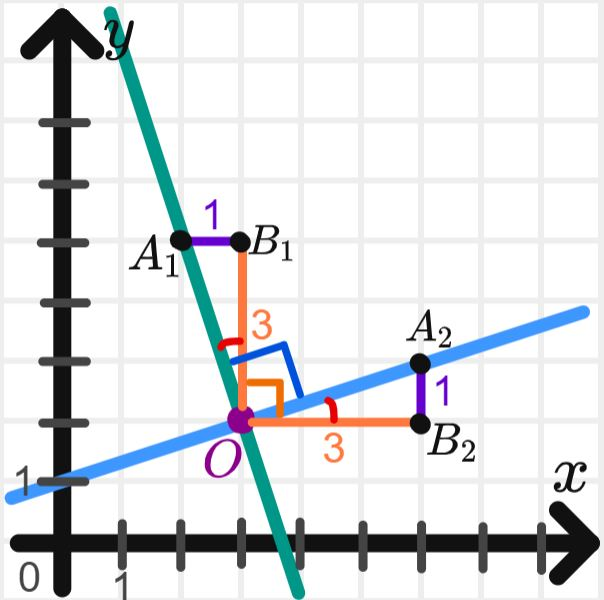
\includegraphics[width=\linewidth]{sol14}\end{figure}\end{minipage}
\end{minipage}
\vspace{-2mm}\\Раз треугольники равны, то равны и их уголки, отмеченные на рисунке красным. Получается, что прямой угол $B_1OB_2$ просто поворачивается влево.\\ И поскольку при повороте угол остаётся прямым, то и угол между указанными прямыми будет прямым и равен 90$^\circ$.}
{Координаты точки пересечения~--- $(3; 2)$, угол между прямыми равен 90$^\circ$.}{Доказательство перпендикулярности опирается на тот факт, что это повёрнутый прямой угол.}
\end{problem}

\begin{problem}{Решение системы линейных уравнений графическим методом.}{8.1.7}{7A red параметр}{(лёгкая)}
{При каком значении $k$ прямые $x + 2y = 5$ и $kx - 6y = 4$ не пересекаются?}
{НаписанноеРешение}
{ВерныйОтвет}{Подсказка}
\end{problem}

\end{document}